% ============================================================
% Section: Method
% ============================================================

\section{Coral: A Framework for Autonomous Multi-Agent Evolution}
\subsection{Preliminaries: Problem Formulation for Open-Ended Discovery}
\label{Sec:method:preliminary}

We consider open-ended discovery tasks, where the optimal solution is unknown and increasingly strong candidate solutions must be discovered through iterative search under evaluator feedback. A task instance is specified by a task description $x$ and an evaluator $E$, where evaluating a candidate solution $y$ returns $E(x,y) := (s,f),$ with $s$ denoting the score of $y$ and $f$ denoting auxiliary feedback such as sub-score breakdowns or textual critique from an LLM-powered evaluator.

Let $\mathcal{M}_t$ denote the shared persistent memory available at search step $t$, such as prior candidate solutions and their evaluation outcomes. At an abstract level, each improvement step consists of four stages:
\squishlisttwo[\arabic*.]
    \item \stage{Retrieve}: construct a working context $\hat{\mathcal{M}}_t$ from $\mathcal{M}_t$;
    \item \stage{Propose}: generate a candidate solution $y_{t+1}$ conditioned on $x$ and $\hat{\mathcal{M}}_t$;
    \item \stage{Evaluate}: obtain score and feedback $(s_{t+1}, f_{t+1}) = E(x, y_{t+1})$;
    \item \stage{Update}: incorporate new information into shared persistent memory to form $\mathcal{M}_{t+1}$.
\squishend
% \paragraph{Autonomous self-evolution.}
% We instead study a setting in which these search decisions are delegated to autonomous agents. At step $t$, an agent may perform \stage{Retrieve} by deciding what information to include in $\hat{\mathcal{M}}_t$, perform \stage{Propose} by generating a candidate $y_{t+1}$ conditioned on that context, and perform \stage{Update} by deciding what information to write back into persistent memory after \stage{Evaluate}. Thus, unlike fixed evolutionary search, the agent participates not only in candidate generation, but also in context construction and memory formation. In the multi-agent setting, multiple autonomous agents interact with the same persistent memory in parallel.
% \subsection{Background: Fixed Search Strategies}

% For an evolution strategy, the search strategy $\pi_{\theta}$ comprises the process of selecting past candidates to improve and proposing new solutions~\citep{liu2026evox}. The majority of existing works~\citep{sharma2025openevolve,novikov2025alphaevolve} adopt a fixed search strategy where $\pi_{\theta}$ is parameterized with fixed values in the form of programmatic rules or heuristics \paul{not clear, give 1 specific example}. Some more recent works~\citep{lange2025shinkaevolve,liu2026evox,cemri2026adaevolve} have made attempts at reducing the rigidness of fixed search strategies by introducing elements of LLM control \paul{also not clear. explain more in the context of the problem statement}. However, they are still fundamentally rule-driven, where each evolution step follows a fixed workflow of candidate selection, solution proposal, evaluation, and feedback generation. We therefore loosely group them under the category of fixed search strategies.

\subsection{From Fixed Search to Autonomous Multi-Agent Evolution}
% \begin{table*}[t]
% \centering
% \caption{Comparison of three paradigms for LLM-based open-ended discovery.}
% \label{tab:paradigm_comparison}
% \small
% \setlength{\tabcolsep}{4pt}
% \renewcommand{\arraystretch}{1.1}
% \begin{tabularx}{\textwidth}{>{\bfseries}p{1.55cm}XXX}
% \toprule
% Stage & Fixed evolutionary search & Autonomous single-agent evolution & Autonomous multi-agent evolution \\
% % \midrule

% Retrieve
% & Context is selected by fixed rules.
% & The agent chooses what prior knowledge to inspect.
% & Each agent retrieves from shared memory. \\

% Propose
% & The model proposes from the given context.
% & The agent plans, implements, debugs, and refines a candidate.
% & Multiple agents propose in parallel. \\

% Evaluate
% & Evaluation is triggered by a fixed loop.
% & The agent decides when to evaluate.
% & Each agent schedules its own evaluations. \\

% Update
% & Memory is updated by fixed rules.
% & The agent decides what to store.
% & Agents write reusable artifacts to shared memory. \\

% \bottomrule
% \end{tabularx}
% \end{table*}


Most prior LLM-based methods for open-ended discovery follow \emph{fixed evolutionary search}, where the four stages in Section~\ref{Sec:method:preliminary} are instantiated by externally specified rules (Figure~\ref{fig:paradigm_comparison}). In this paradigm, \stage{Retrieve} and \stage{Update} are governed by fixed procedures, while the LLM mainly acts in \stage{Propose}, typically generating a candidate from a constructed context in a single forward pass, and \stage{Evaluate} is handled by the task evaluator. For example, in AlphaEvolve~\citep{novikov2025alphaevolve}, the working context $\hat{\mathcal{M}}_t$ is constructed from $\mathcal{M}_t$ using predetermined selection rules inspired by MAP-Elites and island models. This paradigm is effective, but it leaves key search decisions outside the agent. The agent does not decide what evidence to inspect, when to verify intermediate results, how to react to failure, or what knowledge to preserve for reuse. For open-ended discovery, however, these choices are often part of the problem itself.

This motivates \textbf{\emph{autonomous single-agent evolution}}. Here, a single agent controls a much larger portion of the search process: it can decide what to retrieve, when to run local tests, when to invoke the evaluator, and what to write back to persistent memory. The same four stages still apply, but their timing and realization are no longer fixed externally (Figure~\ref{fig:paradigm_comparison}). We further extend this idea to \textbf{\emph{autonomous multi-agent evolution}}, where multiple agents run asynchronously while coordinating through shared persistent memory (Figure~\ref{fig:paradigm_comparison}). Rather than relying on predefined roles or a communication structure, agents interact indirectly through shared persistent memory. This increases exploration diversity and allows multiple agents to inspire each other.

We advocate autonomous multi-agent evolution as a promising paradigm for open-ended discovery and introduce \method{} as a lightweight infrastructure to realize it. \method{} delegates much more of the search process to autonomous agents, while keeping the evaluator as an API accessible to the agent, with the grader details hidden.
This added flexibility also introduces systems challenges: agents must remain persistent over long horizons, avoid drift, accumulate reusable knowledge, and operate safely without overloading compute resources or hacking the evaluator. To address these challenges, \method{} introduces three core mechanisms: shared persistent memory, asynchronous multi-agent organization, and heartbeat-based interventions, along with several execution safeguards (see Appendix~\ref{app:safeguards}).

% Most prior LLM-based methods for open-ended discovery instantiate the four stages in Section~\ref{Sec:method:preliminary} using externally specified search strategies. In these systems, \stage{Retrieve} and \stage{Update} are governed by fixed rules outside the model, while the LLM mainly serves as a proposer during \stage{Propose} to generate a new candidate solution conditioned on a constructed context, usually with a single forward pass. \textbf{Evaluate} is then carried out by the task evaluator. For example, in \emph{AlphaEvolve}~\citep{novikov2025alphaevolve} and \emph{OpenEvolve}~\citep{sharma2025openevolve}, the working context $\hat{\mathcal{M}}_t$ is constructed by selecting historical solutions with a predetermined selection procedure over $\mathcal{M}_t$, inspired by evolutionary mechanisms such as MAP-Elites and island models. The update to memory is likewise rule-based: evaluated solutions are inserted into the population, which consists of all historical attempts and their metadata, such as parent-child relationships and island assignments.

% This paradigm has proven effective, but it also imposes a strong restriction: key decisions remain outside the agent. In particular, the agent does not decide what prior evidence and knowledge to inspect, when to perform intermediate verification, how to interpret failures, or what newly acquired knowledge should be stored for future reuse. Instead, these choices are largely prescribed by an outer-loop controller. For open-ended discovery tasks, however, such decisions are often part of the search problem itself and can substantially affect performance.

% This motivates a more autonomous alternative. In \emph{autonomous single-agent evolution}, a single agent is no longer treated as a local mutation operator inside a fixed search pipeline. Instead, it is allowed to manage a much larger portion of the search process: the agent may decide when to inspect prior knowledge and attempts, when to run local tests, when to invoke the evaluator, and what information to write back to persistent memory. The four stages of \stage{Retrieve}, \stage{Propose}, \stage{Evaluate}, and \stage{Update} still provide a useful abstract decomposition, but their timing, frequency, and realization are specified as overall guidelines rather than being externally constrained.

% We further argue that autonomy should scale horizontally from one agent to many. In \emph{autonomous multi-agent evolution}, multiple such agents run asynchronously, each pursuing its own search trajectory while coordinating indirectly through shared memory. This removes the need for a predefined role decomposition or explicit communication topology. Instead, useful discoveries made by one agent can influence the retrieval, proposal, and update decisions of others through persistent shared artifacts. Compared with single-agent autonomy, this organization increases exploration diversity and enables parallel search while preserving long-horizon knowledge accumulation.

% We advocate autonomous multi-agent evolution as a promising paradigm for open-ended discovery, and introduce \method{} as a lightweight infrastructure for realizing it. Rather than placing language models inside a fixed outer-loop procedure, \method{} delegates a much larger portion of the search process to autonomous agents while retaining the evaluator as a passive API that agents may invoke when needed. As summarized in Table~\ref{tab:paradigm_comparison}, the four stages remain a useful abstraction across fixed search, autonomous single-agent evolution, and autonomous multi-agent evolution, but control over these stages shifts fundamentally across the three paradigms.

% The added flexibility of autonomous multi-agent evolution also introduces new systems challenges: agents must remain alive and sustained throughout the task, avoid instruction forgetting or unproductive drift, reliably accumulate reusable knowledge over long horizons, and ensure that compute resources and the grader are not hacked by increasingly autonomous agents. To address these challenges, \method{} introduces three core mechanisms: persistent shared memory, asynchronous multi-agent organization, and heartbeat-based interventions. We describe these mechanisms next. Additional technical details, including task APIs and system interfaces, are provided in Appendix~\ref{app:implementation}.


% \paragraph{Fixed evolutionary search.}
% Most prior LLM-based evolutionary methods instantiate the four stages above with externally specified search strategies.  Particularly, \stage{Retrieve} and \stage{Update} are governed by fixed rules independent of the proposer, which generates $y_{t+1}$ conditioned on the constructed context $\hat{\mathcal{M}}_t$, typically in a single forward pass. \stage{Evaluate} is then carried out by the evaluator $E$. For example, in \emph{OpenEvolve}~\citep{sharma2025openevolve}, \stage{Retrieve} constructs $\hat{\mathcal{M}}_t$ by applying a predetermined selection procedure over $\mathcal{M}_t$ (based on MAP-Elites and island models) to choose which historical solutions are exposed to the model, and \stage{Update} is a predefined constrained step such that $\mathcal{M}_{t+1}$ contains the evaluated solutions $\{(y_i, s_i, f_i)\}_{i \leq t+1}$ together with their parent-child relationships and island assignments.
% We advocate autonomous multi-agent evolution as a new paradigm for open-ended improvement, and introduce \method{} as the first lightweight infrastructure for realizing it. Rather than placing language models inside a fixed outer-loop search procedure, \method{} delegates a larger portion of the search process to autonomous agents, allowing them to manage all stages of search while accumulating shared knowledge indefinitely. Specifically, as shown in Figure~\ref{fig:paradigm_comparison}, \method{} does not set a hard boundary between \stage{Retrieve}, \stage{Propose}, \stage{Evaluate}, and \stage{Update}. Each \method{} agent may, on its own will, repeatedly research past literature, propose new ideas, conduct experiments to validate the proposal, and update its belief based on the results. While \method{} provides an external evaluator, it is designed as a passive API for the agent to invoke instead of a proactive component of the workflow. In the multi-agent setting, each agent runs asynchronously, pursuing its own search trajectory while coordinating indirectly through shared memory, so that useful discoveries made by one agent can inform the retrieval, proposal, and update decisions of others.

% Specifically, during \textsc{Retrieve}, a \method{} agent may decide to inspect persistent shared memory as it deems fit. During \textsc{Propose}, an agent can reason, implement, debug, and refine candidate solutions within its workspace before deciding what to submit. In \textsc{Evaluate}, the agent may decide when to invoke evaluation, write a summary of the attempt for future reference, and determine how to use the feedback to guide its search. In \textsc{Update}, the agent may reason about the feedback and choose what newly acquired information to write back into persistent memory. In the multi-agent setting, multiple such agents run in parallel, each pursuing its own search trajectory while coordinating indirectly through shared memory, so that useful discoveries made by one agent can inform the retrieval, proposal, and update decisions of others.

% \paul{i like the retrieve, propose, evaluate, update framework up to here. a figure will help left baselines vs right your approach. but starting here, its not clear how the 4 stages in the framework map to the individual contributions below}

% While dismantling the stages offers much more flexibility to the agents, it also introduces challenges in managing the evolution system to ensure agents continuously work together on the task instead of going astray. In the following, we explain how we design the key mechanisms in \method{} to ensure efficient multi-agent evolution. Additional technical details including task APIs and system interfaces are in Appendix~\ref{app:implementation}.

% In the following subsections, we describe the methodological details of the core modules and concepts in \method{}: persistent shared memory, which stores accumulated knowledge \kai{I also agree that we need to link each contributions below to modules mentioned above.}; the heartbeat mechanism, which intervenes to steer agent behavior when needed; multi-agent coordination, which enables agents to explore in parallel while communicating with one another and contributing to shared memory; and execution safeguards, which improve the safety and robustness of the system. Our method is illustrated in Figure~\ref{fig:coral-diagram}. Additional technical and implementation details are provided in the appendix~\textcolor{red}{[appendix reference]}.
% \textbf{Notation:} We denote $N$ as the total number of agents, $t$ as the current step, and $i, j$ as agent indices. For agent $i$, we denote $\mathcal{C}_t^{(i)}$ and $\mathcal{C}_t^{\prime (i)}$ as its local context before and after a heartbeat intervention, respectively. Furthermore, we denote $\mathcal{M}$ as the global shared memory, $\mathcal{W}_t^{(i)}$ as the artifacts written to $\mathcal{M}$ by agent $i$, and $\hat{\mathcal{M}}_t^{(j)}$ as the memory subset retrieved by agent $j$.


% Source: figures/coral_overview.pdf, \label{fig:coral-diagram} in sections/method.tex.
\begin{figure*}[t!]
  \centering
  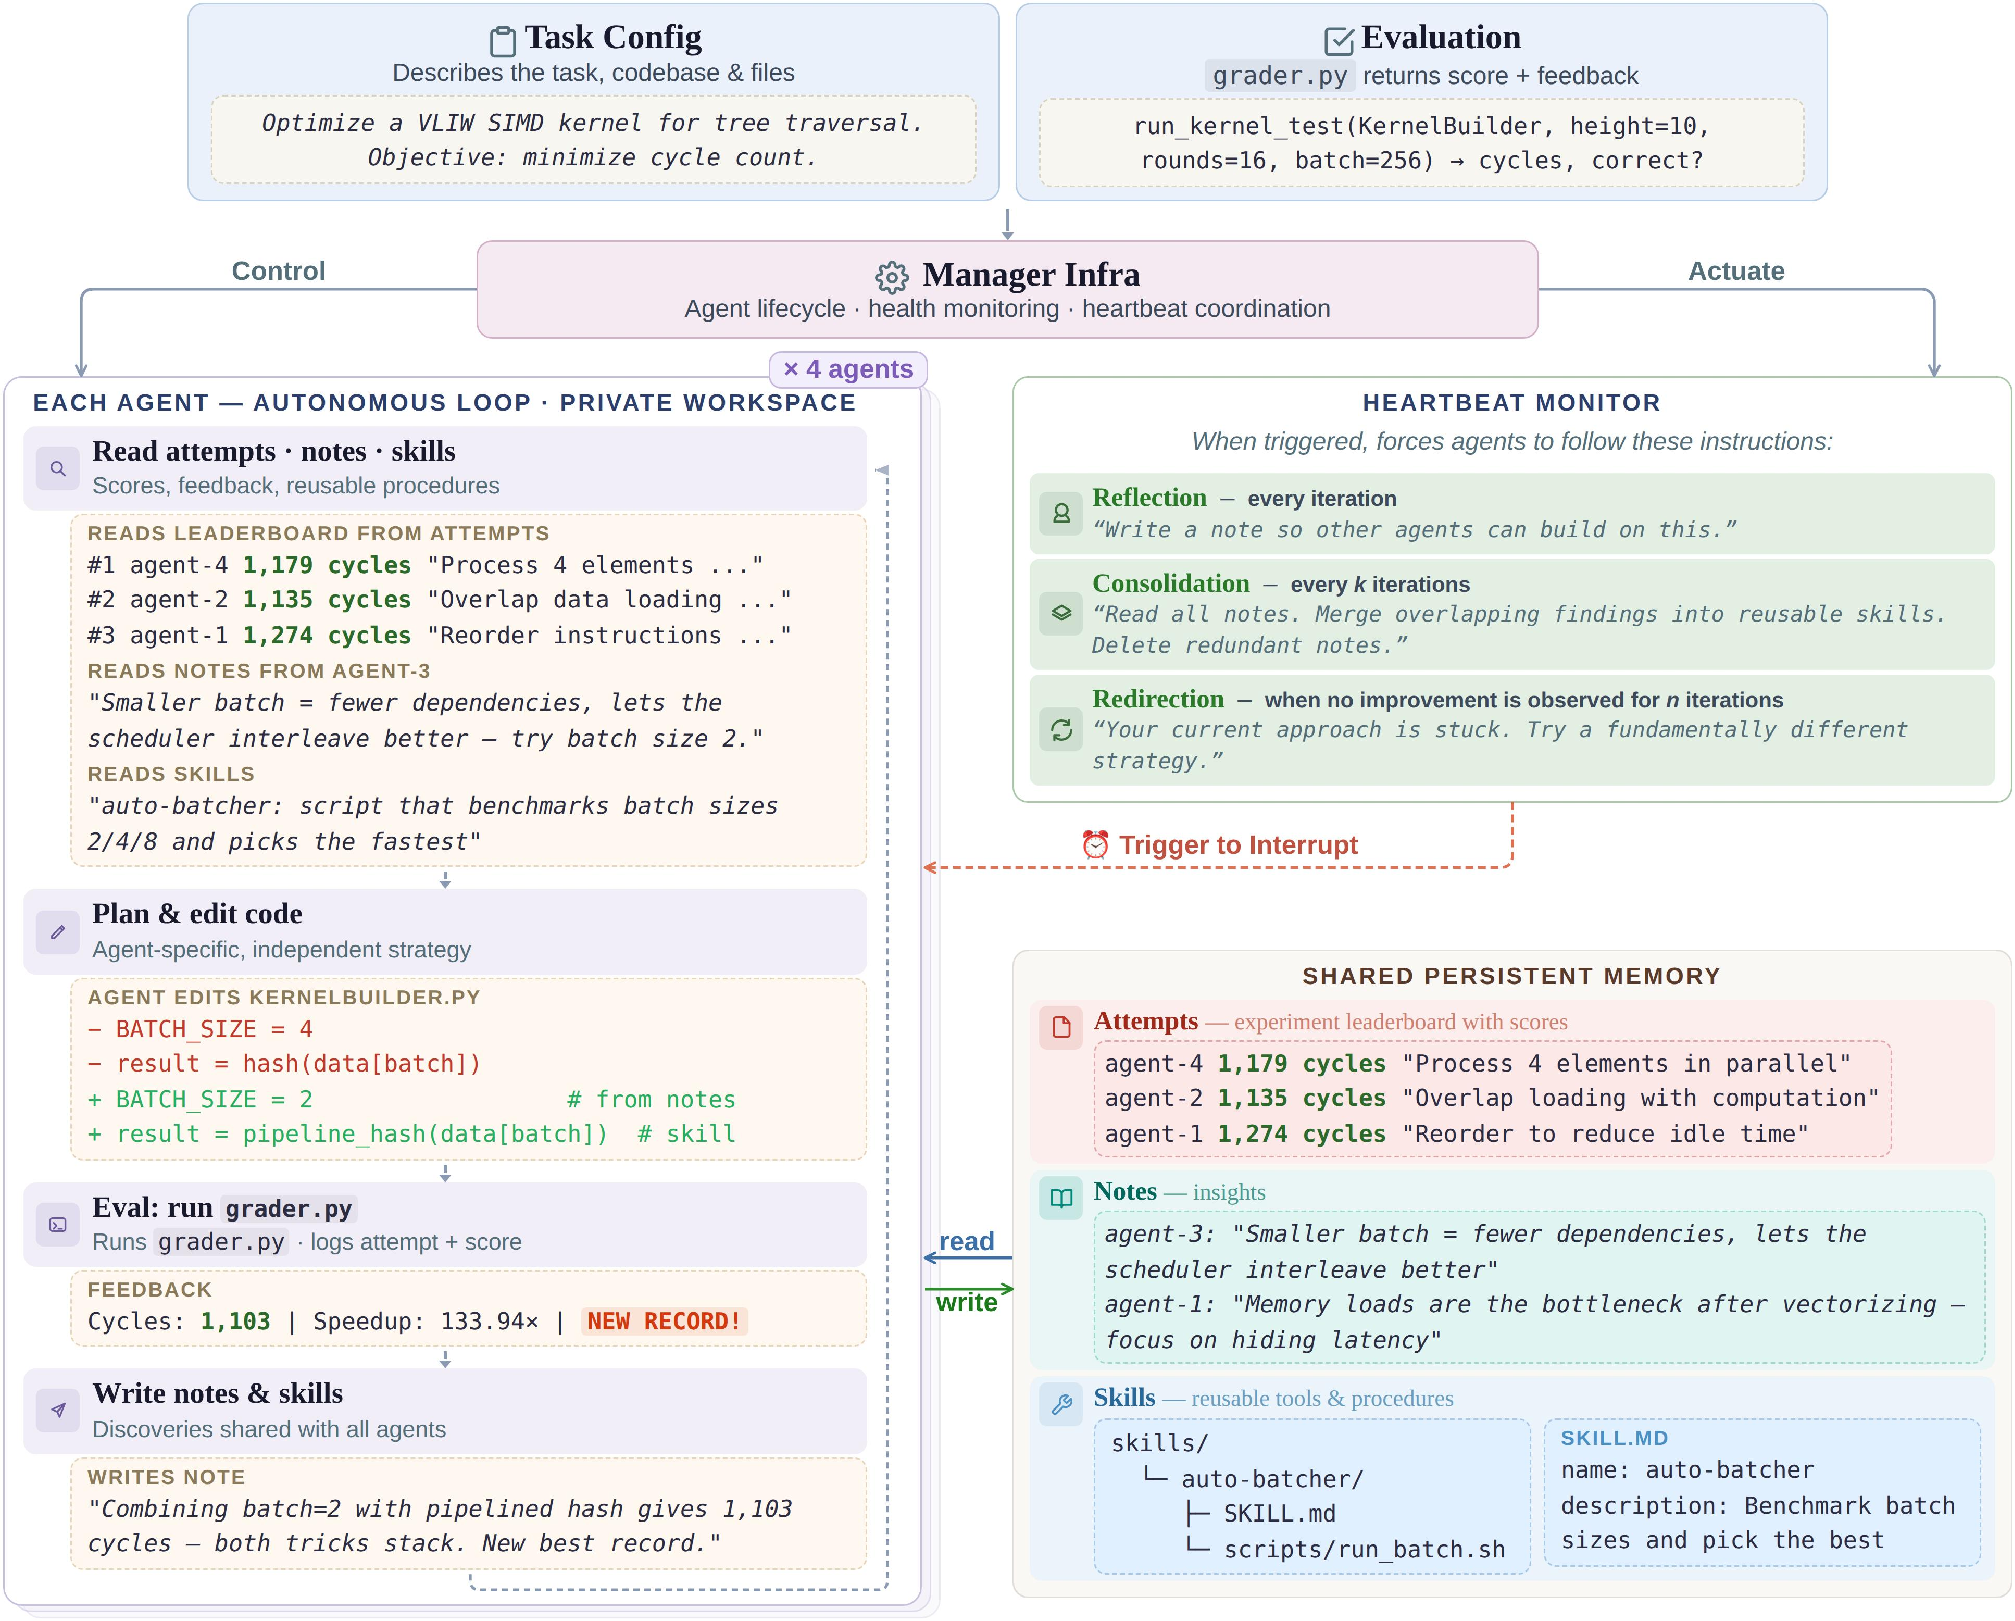
\includegraphics[width=\linewidth]{figures/srcs/02_overview.pdf}
  \vspace{-1pt}
  \caption{Overview of the \method{} framework. Autonomous agents operate in isolated worktrees, iteratively propose and evaluate candidate solutions, and accumulate shared persistent memory (attempts, notes, skills) through a hub. Heartbeat-driven periodic reflections help agents consolidate discoveries and reorient search over long horizons.}
  \label{fig:coral-diagram}
\end{figure*}



\subsection{Core Mechanisms of \method{}}


\textbf{Shared Persistent Memory as File System.}
\method{}'s shared persistent memory $\mathcal{M}$ is structured as a file system with symbolic links to an agent's workspace (also a file system) to maintain consistency. Functioning much like a library, an agent can retrieve and contribute to the shared file system via the \method{} CLI tool (see Appendix~\ref{app:apis}) and directly use \texttt{Bash} tool to access it. Agents can even help `organize` the shared persistent memory by categorizing shared knowledge into sub-folders. This design allows progressive disclosure for agents, saving their contexts, while also being easy to maintain and highly extensible. To provide some bootstrapping structure for the agents, we define three root folders storing different types of knowledge, explained below. Please refer to Appendix~\ref{app:shared_memory} for examples.

% To support long-horizon search, \method{} maintains a persistent shared memory $\mathcal{M}$ that stores artifacts accumulated across attempts and agents. These artifacts include prior attempts together with evaluator outcomes and metadata, as well as knowledge, including failures to avoid, promising directions, intermediate artifacts, and reusable procedures.

% Given the current task context, agent $i$ retrieves a relevant memory context $\hat{\mathcal{M}}_t^{(i)}$ from $\mathcal{M}$ through the \method{} memory APIs, which support retrieval by performance, recency, hybrid query matching, and agent-specific filtering (details in Appendix~\ref{app:apis}). This context may include prior attempts, recent observations, reusable skills, or query-matched artifacts. After producing and evaluating an attempt at local step $t$, agent $i$ may also write a set of artifacts $\mathcal{W}_t^{(i)}$ back to shared memory $\mathcal{M}$, including the attempt itself, distilled notes, and reusable skills. \zijian{The memory is structured as a hierarchical file system in a shared workspace consisting of multiple main folders for different types of artifacts. Each agent has the freedom to read and write to the memory at any time and will have to maintain the filesystem structure of the memory over time. Specifically, we maintain three complementary types of persistent artifacts, each organized as a root folder in the shared workspace.}
% \paul{clarify when agents read and write to mem, size of mem, computational efficiencies and if there are any bottlenecks etc}

\textbf{\texttt{attempts/}} records historical evaluations and solutions. Agents can browse this space to understand high-performing solutions and retrieve their solutions for comparison.

\textbf{\texttt{notes/}} records observations, learnings, and reflections from all agents. Each note is stored as a markdown file in the directory or a subdirectory determined by the agent who creates the note. Agents have full access to all notes.

\textbf{\texttt{skills/}} records reusable procedures, tools, scripts, and implementation patterns transferable across attempts. Following standard practice, a skill consists of a natural-language description (e.g., \texttt{SKILL.md}) together with executable artifacts such as functions and example scripts. Agents are provided with a \texttt{skill\_creator} skill as a guide to create new skills.

% \textbf{Skills} record reusable procedures, tools, scripts, or implementation patterns that may transfer across attempts. Following prior work, a skill may consist of a natural-language description (e.g., \texttt{SKILL.md}) together with executable artifacts such as code snippets, utilities, or example scripts. \zijian{Agents are encouraged (via prompting) to consolidate important and reusable knowledge and create skills for future reference.}
% \paul{clarify how notes and skills are extracted from raw attempt data}

% Implementation-wise, the shared workspace is exposed to each agent's individual workspace through symbolic links. This design combines isolated per-agent workspaces with persistent shared memory for independent execution and shared knowledge reuse.


% \subsection{Heartbeat: Reflection and Redirection}

% To support long-horizon search, \method{} introduces a heartbeat mechanism: a general infrastructure module that intervenes in an agent's ongoing trajectory at selected moments. Heartbeats are designed to mitigate common failure modes of autonomous search, such as \emph{trajectory lock-in}, where an agent stays on an unproductive direction for too long, and \emph{missing externalization}, where useful discoveries remain implicit in a local trajectory and therefore unavailable to future search. Each heartbeat consists of a \emph{trigger} and an \emph{execution}. The trigger determines when intervention occurs, while the execution specifies what the agent does once triggered, such as reassessing recent progress, updating its local plan, or externalizing useful information. 

% In our implementation, we instantiate two heartbeat types. The first is a \emph{periodic reflection heartbeat}, triggered at fixed intervals during an agent's trajectory. Its execution prompts the agent to review recent progress, summarize useful findings, and externalize notes or reusable skills. The second is a \emph{stagnation-triggered redirection heartbeat}, triggered when the agent appears to be stuck, such as after repeated failures, recurring errors, or lack of improvement. Its execution prompts the agent to reassess the current direction and decide whether to continue, revise its strategy, or pivot to a different line of search. These two heartbeat mechanisms help reduce myopic local search and encourages explicit memory formation. 

% While we implement the two heartbeat types above, the abstraction is general and can accommodate other trigger conditions and intervention procedures.


\textbf{Multi-Agent Organization.}
% \paul{add a figure for the multi-agent case showing the agents, shared mem, communication etc} 
\method{} naturally extends from a single autonomous agent to a population of \(N\) agents that run asynchronously. Each agent \(i\) maintains its own local context \(\mathcal{C}_t^{(i)}\) and executes in an isolated workspace while sharing access to the same evaluator and shared persistent memory \(\mathcal{M}\) via symbolic link, i.e., shortcut pointers to the original files. This design allows each agent to freely work on its own without interference.

% multiple search trajectories to unfold concurrently without direct interference.

Unlike many peer-to-peer multi-agent systems where agents directly talk to each other~\citep{langgraph2024}, coordination between agents occurs primarily through shared persistent memory. Similar to the single-agent scenario, each agent may autonomously read and write to a shared workspace. As agents generate attempts, notes, and skills, they write artifacts \(\mathcal{W}_t^{(i)}\) to \(\mathcal{M}\), which may later be retrieved by other agents as part of their own context \(\hat{\mathcal{M}}_t^{(j)}\). % \paul{again clarify when read and write happens and computational size/time of memory} 
This way, one agent's discoveries can influence another agent's future search through what it writes to the shared workspace, without requiring a messaging protocol. 
%\paul{explain what is novel and challenging about all this}
This organization increases exploration diversity by allowing agents to pursue different local directions in parallel while still benefiting from shared accumulation. 

% A centralized shared workspace also encourages all agents to help consolidate and organize the knowledge, leading to greater memory efficiency. In our current implementation, agents are initialized identically. Nevertheless, we observe that role specialization may further diversify exploration and better leverage human prior knowledge. How to assign, adapt, and evolve specialization and coordination strategies in self-evolving multi-agent systems remains an open problem, which we leave for future work. 

% \subsubsection{Execution Safeguards and Implementation}
% \han{see Appendix~\ref{app:safeguards}}
% \zijian{Honestly, this part could be removed if we need to save space}


% Finally, \method{} includes several execution safeguards that improve the robustness of autonomous long-horizon search. First, each agent runs in an isolated workspace, preventing interference across concurrent trajectories and preserving the reproducibility of historical attempts. Second, evaluation is hidden from agents: they may submit candidate solutions and observe evaluator outputs, but they cannot directly inspect or modify the evaluator itself. This separation is important for reducing reward hacking, as agents may otherwise exploit or alter the evaluation procedure to obtain higher scores. Third, agent execution is designed to be persistent: the manager monitors agent health, and if an agent is accidentally terminated, its context is preserved so that execution can resume. Fourth, resources are coordinated through a queuing system that adaptively allocates compute for tasks whose development or evaluation requires substantial resources. \paul{again, explain which of these are new contributions vs standard practices}


\textbf{Heartbeat: Reflection, Consolidation and Redirection.}
As \method{} does not enforce the fixed-search workflow, agents may inadvertently fall into local minima, where they decide to work on micro-optimizations instead of trying out innovative ideas. Agents may also forget to consult and contribute to shared persistent memory. To encourage desirable behavior, \method{} imposes a heartbeat mechanism that functions like a \textit{Reminder App}, periodically prompting the agents to exercise self-reflection and pivoting for new ideas when existing approaches plateau.
% To support long-horizon search, \method{} introduces a heartbeat mechanism: a general infrastructure module that intervenes in an agent's ongoing trajectory at selected moments. Heartbeats are designed to mitigate common failure modes of autonomous search, such as \emph{trajectory lock-in}, where an agent stays on an unproductive direction for too long, and \emph{missing externalization}, where useful discoveries remain implicit in a local trajectory and therefore unavailable to future search.
A heartbeat event may be predefined or created by the agents themselves. Each event is attached to a trigger, which can be the number of intervals, time passed, or a change in eval score.
% \paul{how is the trigger determined? some heuristics? tracking loss function?}
When triggered at step $t$, the heartbeat applies a modification to the agent's local context $\mathcal{C}_t^{(i)} \rightarrow \mathcal{C}_t^{\prime (i)}$ and thereby steers subsequent behavior.

\method{} implements three heartbeat types. The first is a \emph{per-iteration reflection heartbeat}, which encourages the agent to record useful notes during ongoing work. This heartbeat helps the agent capture observations as they arise. The second is a \emph{periodic consolidation heartbeat}, triggered after a fixed number of attempts, which prompts the agent to review progress, organize and refine accumulated notes, and distill reusable procedures into skills. In other words, while the first supports note-taking during work, the second focuses on organizing those notes and building skills from them. The third is a \emph{stagnation-triggered redirection heartbeat}, activated when the agent shows no improvement for several rounds, which prompts it to reassess the current direction and decide whether to continue, revise its strategy, or pivot to a different line of search. Together, these heartbeat mechanisms promote explicit memory formation and reduce myopic local search.

% While we implement the two heartbeat types above, the abstraction is general and can accommodate other trigger conditions and intervention procedures.


% The overall framework is task-agnostic in its evolution loop and memory mechanisms; task-specificity enters primarily through the task and evaluator interface. Full implementation details, including task APIs and system interfaces, are provided in Appendix~\ref{app:implementation}.